\documentclass[]{article}

\usepackage{listings}
\usepackage{color}
\usepackage{placeins}
\usepackage{graphicx}

\graphicspath{ {../media/} }

\definecolor{dkgreen}{rgb}{0,0.6,0}
\definecolor{gray}{rgb}{0.5,0.5,0.5}
\definecolor{mauve}{rgb}{0.58,0,0.82}

\lstset{frame=tb,
  language=C++,
  aboveskip=3mm,
  belowskip=3mm,
  showstringspaces=false,
  columns=flexible,
  basicstyle={\small\ttfamily},
  numbers=left,
  numberstyle=\color{gray},
  keywordstyle=\color{blue},
  commentstyle=\color{dkgreen},
  stringstyle=\color{mauve},
  breaklines=true,
  breakatwhitespace=true,
  tabsize=4
}

\setlength{\parindent}{0pt}
\setlength{\tabcolsep}{.5 cm}

%opening
\title{Causes for Eviction Notices in Assorted Neighborhoods of San Francisco}
\author{
Aitken, Connor\\
\texttt{connor.aitken500@gmail.com}
\and
Cheung, Leon\\
\texttt{leonjcheung@gmail.com}
}

\begin{document}

\maketitle

\begin{abstract}
In recent years, the gentrification of San Francisco has become an increasingly controversial topic for those living in the Bay Area. We have set out to investigate whether the evictions we hear about in the news are morally justifiable or a result of landlords looking to generate greater revenues on their property, due to the great demand for housing. We pulled data from the city's open database initiative \textit{dataSF} and used the C++ Programming Language to statistically analyze the data. We found that there is a veritably greater rate in evictions that we perceive to be motivated by greater potential profits, especially in neighborhoods which are exploding due to the rise of tech companies wishing to maintain offices in San Francisco. With this result in mind, we gain a greater perspective on the objective state of the state of housing in San Francisco.
\end{abstract}

\section{Data Collection}
We downloaded data on eviction statistics from SF OpenData and counted each of the reasons for eviction with a program we designed and created using C++. For some of these expected counts, the data was less than five so we were unable to incorporate it in our testing. After separating the data into eleven districts based off location, we performed $\chi ^{2}$ Data Tests for Homogeneity using the valid counts.
\newpage
\section{Data Context}

Not all neighborhoods of San Francisco are included in the provided data set because some neighborhoods do not contain any rented properties. Below are neighborhoods available to us in the data set, including the District groupings we assigned to them.

\begin{table}[!h]
\begin{tabular}{l | l}
District & Neighborhoods \\
\hline
1 		 & Outer Richmond, Inner Richmond, Lone Mountain/USF \\
2		 & Presidio Heights, Marina, Russian Hill, Pacific Heights \\
3 		 & North Beach, Nob Hill \\
4		 & Sunset/Parkside \\
5		 & Haight Ashbury, Hayes Valley, Western Addition \\
6		 & Tenderloin, South of Market, Financial District/South Beach \\
7		 & Lakeshore \\
8 		 & Noe Valley, Twin Peaks, Glen Park \\
9		 & Portola Heights, Bernal Heights, Mission \\
10 		 & Visitacion Valley, Bayview Hunters Point, Portrero Hill \\
11		 & Oceanview/Merced/Ingleside, Outer Mission, Excelsior \\
\end{tabular}
\caption{Available Neighrbohoods and Their Districts}
\end{table}

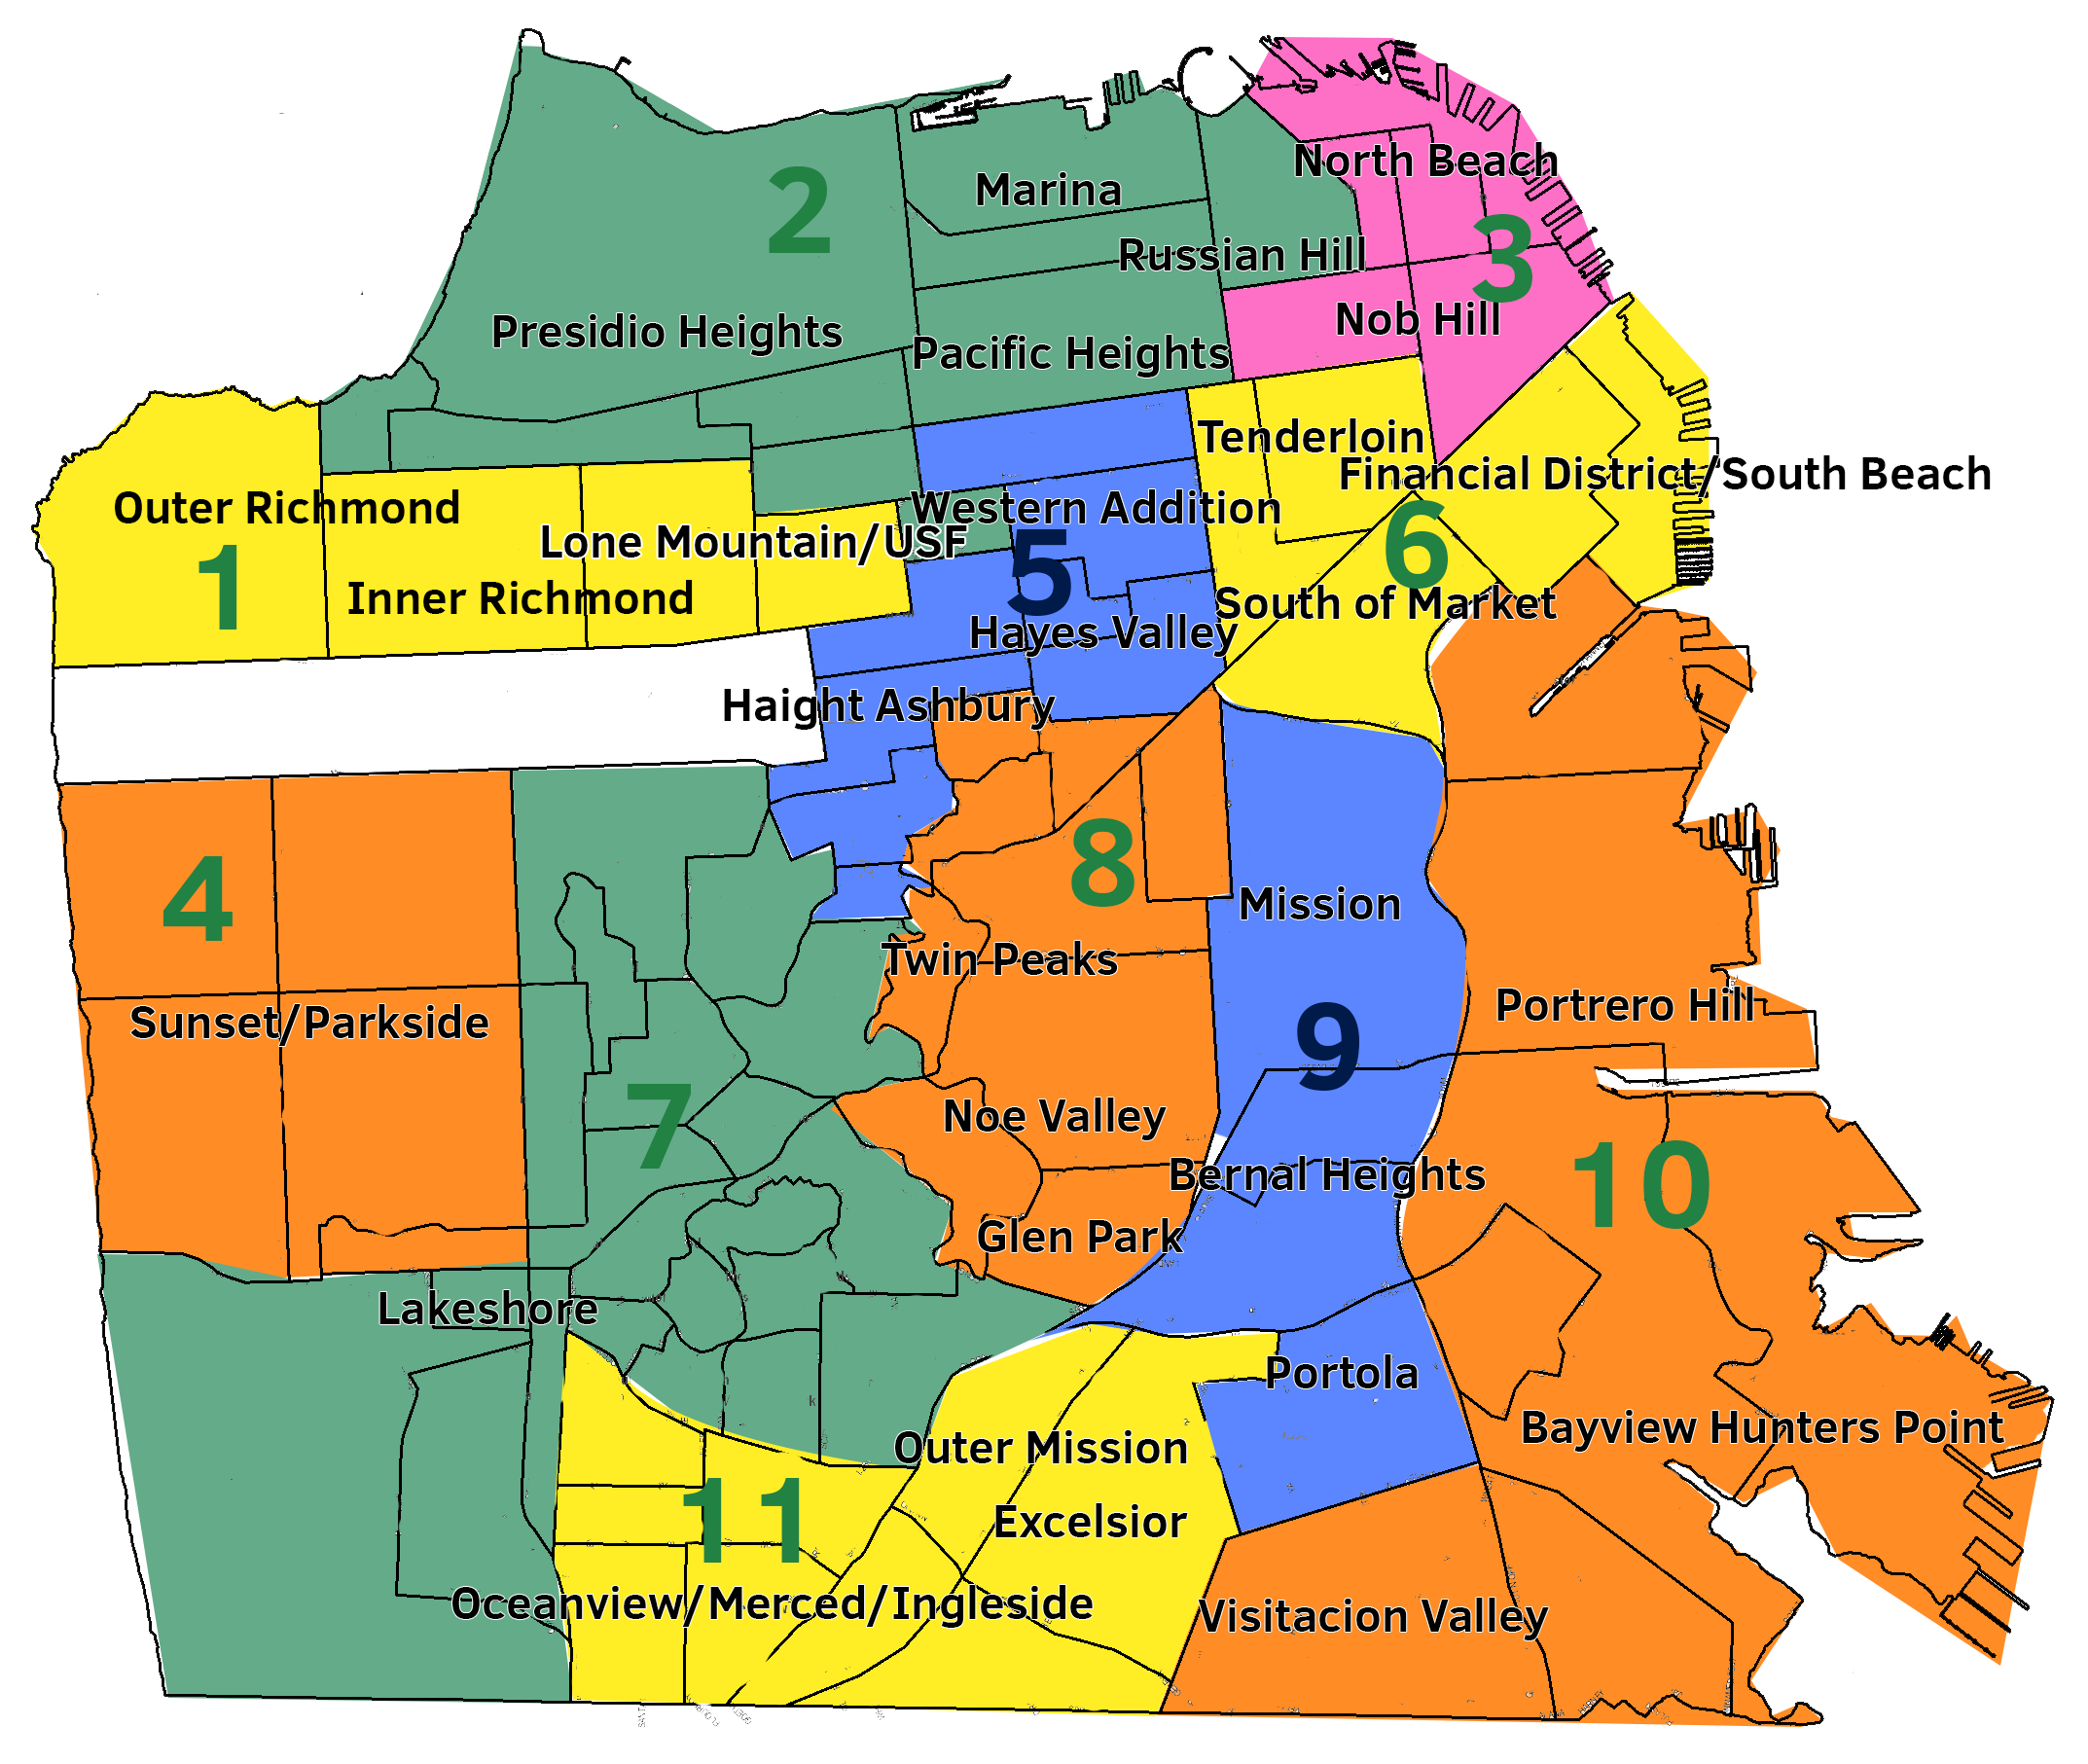
\includegraphics[height=10cm]{legitmap}

Some neighborhoods and eviction reasons contained far too little data to produce anything meaningful. They are listed below.

\begin{table}[!h]
\begin{tabular}{l | l}
Category & Removed \\\hline
Reasons  & Other, lead remediation, good samaritan \\
Neighborhoods & Presidio, Seacliff, Mission Bay, Golden Gate Park \\
Time period & All eviction notices before January 2005 \\
\end{tabular}
\caption{Available Neighrbohoods and Their Districts}
\end{table}

Instead of running one $\chi ^{2}$ test on all of the eviction reasons, we decided to group the reasons into four categories.

\begin{table}[!h]
\begin{tabular}{l | l}

	Tenant Action    	& Non Payment, Breach of Contract, Nuisance, Illegal, 	  \\
						& Unapproved Subtenant, Late Payment			    	  \\\\
	Landlord Action     & Fail to Sign Renew, Owner Move-in, Capital Improvement, \\ 
						& substantial rehab, roommate same unit 				  \\\\
	Development    		& Demolition, Ellis Act Withdrawal, Condo Conversion      \\\\  
	Just Cause    		& Non Payment, Late Payment, Breach of Contract, 		  \\ 
						& Owner Move-in, Capital Improvement, Ellis Act Withdrawal, \\ 
						& Nuisance, Illegal, Demolition 						  \\	
	\end{tabular}
\caption{Eviction Reason Categories}
\end{table}

\section{Inferential Procedures}
\subsection{District 1}

\begin{table}[!h]
\centering
\begin{tabular}{l | l}
Neighborhoods & Inner Richmond, Lone Mountain/USF, Outer Richmond \\
\end{tabular}
\end{table}
\FloatBarrier

\begin {table}[!h]
\centering
\begin{tabular}{l | r | r | r}
	
	Reason	&  $\chi ^{2}$ & df & p-Value \\
	Tenant Action 		   &  15.1570  & 10  & 0.1264  \\
	Landlord Action	       &  10.4669  & 6   & 0.1062 \\
	Development			   &  0.9854   & 2   & 0.6110 \\
	Just Cause Removal	   &  39.9610  & 16  & 0.0008 \\
\end{tabular} \newline
\end{table}
\FloatBarrier


For District 1, there was homogeneity shown in all areas besides "Just Cause Removal". This may be because of Lone Mountain's low nonpay component of 0.4827 or Inner Richmond's high ownermovein component of 4.1747.

\newpage
\subsection{District 2}
\begin{table}[!h]
	\centering
	\begin{tabular}{l | l}
		Neighborhoods & Presidio Heights, Marina, Russian Hill, Pacific Heights \\
	\end{tabular}
\end{table}
\FloatBarrier

\begin {table}[!h]
\centering
\begin{tabular}{l | r | r | r}
	
	Reason	&  $\chi ^{2}$ & df & p-Value \\
	Tenant Action 		 & 45.4120 &  15   & 0.0001 		\\
	Landlord Action	     & 11.8037 &  6     &  	0.0665	\\
	Development			 & 0.3398 &  6    &  0.9993		\\
	Just Cause Removal	 & 127.1146   &  24 &  	0.0000		\\
\end{tabular} \newline
\end{table}
\FloatBarrier

For District 2, homogeneity was only shown in "Just Cause Removal" and "Tenant Action." Pacific Heights' high nonpayment component of 11.6593 likely impacts both of these sections.

\subsection{District 3}

\begin{table}[!h]
	\centering
	\begin{tabular}{l | l}
		Neighborhoods & North Beach, Nob Hill \\
	\end{tabular}
\end{table}
\FloatBarrier

\begin {table}[!h]
\centering
\begin{tabular}{l | r | r | r}
	
	Reason	&  $\chi ^{2}$ & df & p-Value \\
	Tenant Action 		  & 8.0298 &  5  &  0.1955    \\
	Landlord Action	      & 2.2699 &  3  &  0.7037    \\
	Development			  & 0.0000 &  1  &  1.0000    \\
	Just Cause Removal	  & 19.6549 &  8  &  0.0117    \\
\end{tabular} \newline
\end{table}
\FloatBarrier

For District 4, Homogeneity was shown in all categories but "Just Cause Removal." This may be because of North Beach's almost double nonpayment and ellisactwithdrawl compared to Nob Hill's components.

\subsection{District 5}

\begin{table}[!h]
	\centering
	\begin{tabular}{l | l}
		Neighborhoods & Haight Ashbury, Hayes Valley, Western Addition \\
	\end{tabular}
\end{table}
\FloatBarrier

\begin {table}[!h]
\centering
\begin{tabular}{l | r | r | r}
	
	Reason				&  $\chi ^{2}$ & df & p-Value \\
	Tenant Action 		   &  32.4910   &  10 & 0.0003 \\
	Landlord Action	       &  10.6710  & 6  & 0.0991 \\
	Development			   &  0.9271  &  4 & 0.9206 \\
	Just Cause Removal	   &  111.3054  & 16  & 0.0000 \\
\end{tabular} \newline
\end{table}
\FloatBarrier

Homogeneity is shown in all categories besides "Tenant Action" and "Just Cause Removal." In regards to "Tenant Action," Hayes Valley high nonpayment component of 6.8882 and Western Addition's high nuisance component of 6.3202 likely contribute to the lack of homogeneity, and in "Just Cause Removal," Western Addition's extremely low capital improvement component of 0.1674 does not correlate with the next lowest in Western Addison of 14.6997.

\subsection{District 6}


\begin{table}[!h]
	\centering
	\begin{tabular}{l | l}
		Neighborhoods & Tenderloin, South of Market, Financial District/South Beach  \\
	\end{tabular}
\end{table}
\FloatBarrier

\begin {table}[!h]
\centering
\begin{tabular}{l | r | r | r}
	
	Reason				 &  $\chi ^{2}$ & df & p-Value \\
	Tenant Action 		   &  46.9304  & 4  & 0.0000 \\
	Landlord Action	       &  0.0000  & -2  & 1.0000 \\
	Development			   &  0.0000  & -2  & 1.0000 \\
	Just Cause Removal	   &  63.8182  & 4  & 0.0000 \\
\end{tabular} \newline
\end{table}
\FloatBarrier

Homogeneity is shown in the categories of "Tenant Action" and "Just Cause Removal." This may be because of Financial District/South Beach's high nuisance component of 8.1637 and its low nonpayment component of 6.3031.

\subsection{District 8}

\begin{table}[!h]
	\centering
	\begin{tabular}{l | l}
		Neighborhoods & Noe Valley, Glen Park, Twin Peaks
	\end{tabular}
\end{table}
\FloatBarrier

\begin {table}[!h]
\centering
\begin{tabular}{l | r | r | r}
	
	Reason				 &  $\chi ^{2}$ & df & p-Value \\
	Tenant Action 		   &  10.5992  &  2 & 0.0050 \\
	Landlord Action	       &  1.1193  &  0 & 1.0000 \\
	Development			   &  1.1314  & 0  & 1.0000 \\
	Just Cause Removal	   &  37.6297  &  6 & 0.0000 \\
\end{tabular} \newline
\end{table}
\FloatBarrier

Homogeneity is shown in the categories of "Tenant Action" and "Just Cause Removal." The reasons for this in "Tenant Action" may be Glen Park's low nuisance component of 0.2598, and in "Just Cause Removal" it may be because of Glen Park's high breach value of 5.9563 and low ellisactwithdrawl of 0.0003.

\subsection{District 9}

\begin {table}[!h]
\centering
\begin{tabular}{l | l}
	Neighborhoods &  Portola, Bernal Heights, Mission
\end{tabular}
\begin{tabular}{l | r | r | r}
	
	Reason				 &  $\chi ^{2}$ & df & p-Values\\
	Tenant Action 		   & 12.4686   &  6 & 0.0523 \\
	Landlord Action	       &  1.3052  & 2  & 0.5207 \\
	Development			   &  19.1170  & 0  & 1.0000 \\
	Just Cause Removal	   &  133.8546  & 12  & 0.0000 \\
\end{tabular} \newline
\end{table}
\FloatBarrier

Homogeneity is shown in all areas besides "Just Cause Removal." This is most likely because Portola has an exremently high ellisactwithdrawl value of 20.7812. The next highest is only 4.3994 in Mission.  

\subsection{District 10}

\begin {table}[!h]
\centering
\begin{tabular}{l | l}
	Neighborhoods & Visitacion Valley, Bayview Hunters Point, Portrero Hill
\end{tabular}
\begin{tabular}{l | r | r | r}
	
	Reason				 &  $\chi ^{2}$ & df & p-Value \\
	Tenant Action 		   &  3.8906  &  4  & 0.4210 \\
	Landlord Action	       &  1.5766  &  1  & 0.3173 \\
	Development			   &  0.0000  &  -1  & 1.0000 \\
	Just Cause Removal	   &  8.6997  &  5  & 0.1640 \\
\end{tabular} \newline
\end{table}
\FloatBarrier

District 10 has evidence of homogeneity. Each of the reason's p-Value is above 0.05.

\subsection{District 11}

\begin{table}[!h]
	\centering
	\begin{tabular}{l | l}
		Neighborhoods &  Oceanview/Merced/Ingleside, Outer Mission, Excelsior  \\
	\end{tabular}
\end{table}
\FloatBarrier

\begin {table}[!h]
\centering
\begin{tabular}{l | r | r | r}
	
	Reason				 &  $\chi ^{2}$ & df & p-Value \\
	Tenant Action 		   &  23.1291  &  8  & 0.0032 \\
	Landlord Action	       &   2.2277 &  2  & 0.3283 \\
	Development			   &  3.8359  &  2  & 0.1469 \\
	Just Cause Removal	   &  30.6304  &  14  & 0.0062 \\
\end{tabular} \newline
\end{table}
\FloatBarrier

Only "Tenant Action" and "Just Cause Removal" do not show evidence of homogeneity in District 11. For "Tenant Action," this may be because of Outer Mission's high breach component of 5.7766, and in "Just Cause Removal" it could be because of the Oceanview/Merced/Ingleside's nuisance component of 0.0220.

\newpage
\subsection{District 3 vs. District 6}
\begin{table}[h]
\centering
\begin{tabular}{l | l}
Neighborhoods &  North Beach, Nob Hill, 			 \\ 
			  &  Tenderloin, South of Market, Financial Ditsrict/South Beach \\
\end{tabular}
\end{table}

\begin {table}[h]
\centering
\begin{tabular}{l | r | r | r}	
Reason				 &  $\chi ^{2}$ & df    & p-Value   \\
Tenant Action 		 &  50.260      &  8    & 0.0000    \\
Landlord Action	     &  na          &  na   & na        \\
Development			 &  na          &  na   & na        \\
Just Cause Removal	 &  341.925     &  12   & 0.0000    \\
\end{tabular} \newline
\end{table}

The Landlord Action and Development categories yielded no results because we were unable to perform the test, due to the expected counts condition. We were successful in running a test that produced clear results for the Tenant Action and Just Cause Removal categories, however. The greatest component of the Tenant Action category was the Non Payment reason for District 6, which we think is likely due to rising rents in the Tenderloin neighborhood.
\newline\newline
We saw clear non-homogeneity in the Just Cause Removal test, where the p-Value approached zero. Here, the largest components for both District 3 and District 6 were due to the Ellis Act Withdrawal eviction reason, with components of 144.9395 and 81.4898, respectively. This indicates that an immense amount of landlords are removing their property from the rental market for other uses.

\subsection{District 1 vs. District 4}
\begin{table}[!h]
\centering
\begin{tabular}{l | l}
Neighborhoods &  Outer Richmond, Inner Richmond, Lone Mountain/USF,  \\ 
			  &  Sunset/Parkside \\
\end{tabular}
\end{table}

\begin {table}[!h]
\centering
\begin{tabular}{l | r | r | r}	
Reason				 &  $\chi ^{2}$ & df    & p-Value   \\
Tenant Action 		 &  13.3248     & 12    & 0.3459    \\
Landlord Action	     &  8.6267      & 6     & 0.1957    \\
Development			 &  78.7158     & 3     & 0.0000    \\
Just Cause Removal	 &  106.561     & 24    & 0.0000    \\
\end{tabular} \newline
\end{table}

Between these two districts, we see that the evictions due to renter and landlord action occur at relatively the same rate relative to the size of each district. It may be interesting to note that for the Landlord Action category, much of the statistic was made of one component: the Capital Improvement reason for District 4 at 5.2804, which suggests that in the Sunset/Parkside neighborhood landlords are more likely to make significant improvements on their apartments, which temporarily evict tenants from their rooms.
\newline\newline
For reasons which we grouped under Development, these produced components with large values. The greatest contributor to the Development reason was from the Demolition reason from District 4 at 39.8452. This altogether may not be too unexpected, because, from anecdotal experience, there are many buildings which have fallen into disarray or may not be within building code in the first place.
\newline\newline
When we study the Just Cause Removal test, we find more clear differences between these two districts. Both of the largest components of the test statistic resulted from District 4, in the Demolition and Ellis Act Withdrawal reasons, at 47.078 and 15.015 respectively. 

\subsection{District 3 vs. District 5}
\begin{table}[!h]
\centering
\begin{tabular}{l | l}
Neighborhoods &  North Beach, Nob Hill,  \\ 
			  &  Haight Ashbury, Hayes Valley, Western Addition \\
\end{tabular}
\end{table}

\begin {table}[!h]
\centering
\begin{tabular}{l | r | r | r}	
Reason				 &  $\chi ^{2}$ & df    & p-Value   \\
Tenant Action 		 &  9.7614      & 16    & 0.8788    \\
Landlord Action	     &  0.9936      & 8     & 0.9983    \\
Development			 &  0.5791      & 4     & 0.9654    \\
Just Cause Removal	 &  117.5088    & 28    & 0.0000    \\
\end{tabular} \newline
\end{table}

Upon examining the p-Values for each of these tests, it is immediately apparent that these two districts are quite homogenous to each other, at p-Values above 0.85 for Tenant Action, Landlord Action, and Development. However, we see a departure from homogeneity in the Just Cause Removal test, which we could see as a unification of all three of these tests.
\newline\newline
As we parse the components of the Just Cause Removal test, we find that three key components make up the bulk of the test statistic. For District 3, it is the Ellis Act Withdrawal reason, at a value of 39.0179, and for District 5, it is the Owner Move In and Capital Improvement reasons at 30.4084 and 21.7573 respectively that contribute the most. Perhaps District 5 is an attractive place for landlords to find to live in their apartment property, and it is possible that in District 3, landlords are liquidating their property in anticipation of higher profits outside of the rental market.

\subsection{District 5 vs. District 6}
\begin{table}[!h]
\centering
\begin{tabular}{l | l}
Neighborhoods & Haight Ashbury, Hayes Valley, Western Addition\\
			  & Tenderloin, South of Market  \\ 
\end{tabular}
\end{table}

\begin {table}[!h]
\centering
\begin{tabular}{l | r | r | r}	
Reason				 &  $\chi ^{2}$ & df    & p-Value   \\
Tenant Action 		 &  45.3672     & 10    & 0.0000    \\
Landlord Action	     &  na          & na    & na        \\
Development			 &  na          & na    & na        \\
Just Cause Removal	 &  407.8489    & 20    & 0.0000    \\
\end{tabular} \newline
\end{table}

For Landlord Action and Development, we could not run the tests because we had expected counts less than 5.
\newline\newline
In the Tenant Action test, we find a clear departure from homogeneity between District 5 and District 6, suggesting a difference in the type of renters between these two areas. Indeed, we can see that District 6 contributes much to the final test statistic, with the two reasons Non Payment and Nuisance at 16.0512 and 21.4209 respectively, suggesting that it may not be advantageous for landlords to hold a property in this area relative to District 5.
\newline\newline
In the Just Cause Removal test, the largest departures from homogeneity are revealed in the components Owner Move In of District 5, and Nuisance and Owner Move In of District 6, at 133.2342, 68.6161, and 61.3065.


\section{Conclusion}
Through our multiple studies, we found that most districts were homogenous except for when we tested for the Tenant Action and Just Cause Removal categories, which suggests that there were a higher amount of renter evictions due to the fault of the renter, and for reasons that the City of San Francisco defines as "just." In our inter-district analyses, we found that there were significant differences between the relative frequencies of each eviction reason, most prominently the Ellis Act Withdrawal was invoked in some neighborhoods far more than others. We can take the information we have learned and apply it in context with the news articles that we read about the housing crisis in San Francisco.

\newpage
\appendix
\section{Source code}
\begin{lstlisting}
#include <EvictionNotice.hpp>
#include <algorithm>
#include <json/json.h>
#include <iostream>
#include <fstream>
#include <streambuf>
#include <map>
#include <vector>
#include <StatFunctions.hpp>

std::string getJSON(const std::string& filename)
{
    std::ifstream file(filename);

    std::string str;
    file.seekg(0, std::ios::end);
    str.reserve(file.tellg());
    file.seekg(0, std::ios::beg);

    str.assign((std::istreambuf_iterator<char>(file)),
                std::istreambuf_iterator<char>());

    return str;

}

std::vector<NeighborhoodCounts> selectColumns(
    const std::vector<Indices>& columns
  , std::vector<NeighborhoodCounts> counts)
{
    std::for_each (counts.begin(), counts.end(),
        [&] (NeighborhoodCounts& row) {
            for (int i = 0; i < row.counts.size(); i++)
            {
                bool selected = false;
                for (int j = 0; j < columns.size(); j++)
                {
                    if (i == columns[j])
                    {
                        selected = true;
                    }
                }
                if (!selected)
                    row.counts[i] = 0;
            }           
        }
    );
    return counts;
}

std::vector<std::vector<Json::Value>> generateRawNotices(const Json::Value& data)
{
    std::vector<std::vector<Json::Value>> raws;
    for (unsigned int i = 0; i < data.size(); i++)
    {
        raws.push_back(std::vector<Json::Value>());
        for (auto it = data[i].begin(); it != data[i].end(); ++it)
        {
            raws[i].push_back(*it);
        }
    }
    return raws;
}

bool contains(const std::vector<std::string>& vec, const std::string str)
{
    for (auto &e : vec)
        if (e.compare(str) == 0) return true;

    return false;
}

std::map<std::string, std::vector<EvictionNotice>> convertRawToBools(
    std::vector<std::vector<Json::Value>> raws)
{
    enum Columns
    {
        ADDRESS = 9, CITY, STATE, ZIP,
        DATE,
        NON_PAYMENT,
        BREACH,
        NUISANCE,
        ILLEGAL,
        FAIL_SIGN_RENEW,
        ACCESS_DENIAL,
        UNAPPROVED_SUBTENANT,
        OWNER_MOVE_IN,
        DEMOLITION,
        CAPITAL_IMPROVEMENT,
        SUBSTANTIAL_REHAB,
        ELLIS_ACT_WITHDRAWAL,
        CONDO_CONVERSION,
        ROOMMATE_SAME_UNIT,
        OTHER,
        LATE_PAY,
        LEAD_REMEDIATION,
        DEVELOPMENT,
        GOOD_SAMARITAN,
        CONSTRAINTS,
        CONSTRAINTS_DATE, SUPERVISOR,
        NEIGHBORHOOD,
        COORDINATES
    };

    std::map<std::string, std::vector<EvictionNotice>> neighborhoodNotices;

    //parse out all entries not wanted and columns and convert to bool
    for (const std::vector<Json::Value> &columns : raws)
    {
        if (columns[DATE].asString().compare("2005-01-01T00:00:00") < 0) //only entries recent 10 years
            continue;
        std::string neighName = columns[Columns::NEIGHBORHOOD].asString();

        EvictionNotice notice;

        for (int i = 0; i < notice.reasons.size(); i++)
        {
            notice.reasons[i] = columns[i + 14].asBool();
        }
        neighborhoodNotices[columns[Columns::NEIGHBORHOOD].asString()].push_back(notice);
    }

    return neighborhoodNotices;
}

Indices getIndex(const std::string& reason)
{
    if (reason.compare("NON_PAYMENT") == 0) return NON_PAYMENT;
    if (reason.compare("BREACH") == 0) return BREACH;
    if (reason.compare("NUISANCE") == 0) return NUISANCE;
    if (reason.compare("ILLEGAL") == 0) return ILLEGAL;
    if (reason.compare("FAIL_SIGN_RENEW") == 0) return FAIL_SIGN_RENEW;
    if (reason.compare("ACCESS_DENIAL") == 0) return ACCESS_DENIAL;
    if (reason.compare("UNAPPROVED_SUBTENANT") == 0) return UNAPPROVED_SUBTENANT;
    if (reason.compare("OWNER_MOVE_IN") == 0) return OWNER_MOVE_IN;
    if (reason.compare("DEMOLITION") == 0) return DEMOLITION;
    if (reason.compare("CAPITAL_IMPROVEMENT") == 0) return CAPITAL_IMPROVEMENT;
    if (reason.compare("SUBSTANTIAL_REHAB") == 0) return SUBSTANTIAL_REHAB;
    if (reason.compare("ELLIS_ACT_WITHDRAWAL") == 0) return ELLIS_ACT_WITHDRAWAL;
    if (reason.compare("CONDO_CONVERSION") == 0) return CONDO_CONVERSION;
    if (reason.compare("ROOMMATE_SAME_UNIT") == 0) return ROOMMATE_SAME_UNIT;
    if (reason.compare("OTHER") == 0) return OTHER;
    if (reason.compare("LATE_PAY") == 0) return LATE_PAY;
    if (reason.compare("LEAD_REMEDIATION") == 0) return LEAD_REMEDIATION;
    if (reason.compare("DEVELOPMENT") == 0) return DEVELOPMENT;
    if (reason.compare("GOOD_SAMARITAN") == 0) return GOOD_SAMARITAN;
}

bool neighborhoodMode = false;
bool columnMode = false;
bool districtMode = false;

void parseArgs(std::string& filename
             , std::vector<std::string>& neighs
             , std::vector<Indices>& cols
             , std::vector<std::string>& dists
             , int argc
             , const char* argv[])
{
    const std::string NEIGH_SELECTOR = "-n";
    const std::string COL_SELECTOR   = "-c";
    const std::string DISTR_SELECTOR = "-d";

    if (argc > 1)
    {
        filename = argv[1];
        for (int i = 2; i < argc; i++)
        {
            std::string arg = argv[i];

            if (arg.compare(NEIGH_SELECTOR) == 0)
            {
                neighborhoodMode = true;
                columnMode = false;
                districtMode = false;
            }
            else if (arg.compare(COL_SELECTOR) == 0)
            {
                neighborhoodMode = false;
                columnMode = true;
                districtMode = false;
            }
            else if (arg.compare(DISTR_SELECTOR) == 0)
            {
                neighborhoodMode = false;
                columnMode = false;
                districtMode = true;
            }

            if (neighborhoodMode)
            {
                if (arg.compare(NEIGH_SELECTOR) != 0)
                    neighs.push_back(arg);
            }
            else if (columnMode)
            {
                if (arg.compare(COL_SELECTOR) != 0)
                    cols.push_back(getIndex(arg));
            }
            else if (districtMode)
            {
                if (arg.compare(DISTR_SELECTOR) != 0)
                    dists.push_back(arg);
            }
        }
    }
}

std::map<std::string, NeighborhoodCounts> createCounts(
    std::map<std::string, std::vector<EvictionNotice>> notices
  , std::vector<std::string> selectedNeighborhoods)
{
    std::map<std::string, NeighborhoodCounts> neighborhoodsCounts;

    auto it = notices.begin();
    auto itend = notices.end();
    for (; it != itend; ++it)
    {
        std::string name = it->first;

        if (!contains(selectedNeighborhoods, name)) continue;

        neighborhoodsCounts[name].neighborhoodName = name;  //for converting map to vec later
        for (auto jt = it->second.begin(); jt != it->second.end(); ++jt)
        {
            for (int i = 0; i < jt->reasons.size(); i++)
            {
                if (jt->reasons[i])
                {
                    neighborhoodsCounts[name].counts[i]++;
                }
                    
            }
        }
    }

    return neighborhoodsCounts;
}

std::vector<NeighborhoodCounts> mapToVec(
    const std::map<std::string, NeighborhoodCounts>& other)
{
    std::vector<NeighborhoodCounts> finalCounts;
    for (auto &e : other)
    {
        finalCounts.push_back(e.second);
    }
    return finalCounts;
}

int main(int argc, const char* argv[])
{
    std::string evictionFilename = "eviction-notices.json";
    std::vector<std::string> selectedNeighborhoods;
    std::vector<Indices> selectedColumns;
    std::vector<std::string> selectedDistricts;

    parseArgs(evictionFilename, selectedNeighborhoods, selectedColumns, selectedDistricts, argc, argv);

    std::string evictions = getJSON(evictionFilename);

    Json::Value root;
    Json::Reader reader;

    reader.parse(evictions, root);

    Json::Value data = root.get("data", "error");

    std::vector<std::vector<Json::Value>> rawNotices = generateRawNotices(data);
    std::map<std::string, std::vector<EvictionNotice>> parsedNotices = convertRawToBools(rawNotices);
    
    //TODO iterate here and generate all of our chis
    std::map<std::string, NeighborhoodCounts> mappedCounts = createCounts(parsedNotices, selectedNeighborhoods);
    std::vector<NeighborhoodCounts> counts = mapToVec(mappedCounts);

    auto selectedColumnCounts = selectColumns(selectedColumns, counts);

    int df = 0;
    double chi = chiSquareStatistic(selectedColumnCounts, df, selectedDistricts);
    double pVal = chiAreaRight(chi, df);
    std::cout << "chi,"   << chi 
              << ",df,"   << df
              << ",pVal," << pVal
              << std::endl;
}
\end{lstlisting}

\end{document}
